\documentclass{beamer}
\usepackage{fancyvrb}
\usepackage{hyperref}
\usepackage{tikz}
\usepackage{tikz-qtree}

\usepackage{graphicx}


\newcommand{\bi}{\begin{itemize}}
\newcommand{\li}{\item}
\newcommand{\ei}{\end{itemize}}

\newcommand{\sect}[1]{
\section{#1}
\begin{frame}[fragile]\frametitle{#1}
}

\mode<presentation>
{
%  \usetheme{Madrid}
  % or ...

%  \setbeamercovered{transparent}
  % or whatever (possibly just delete it)
}

\usepackage[english]{babel}

\usepackage[latin1]{inputenc}

\title[RPN Calculator]
{
RPN Calculator
}

\subtitle{} % (optional)

\author[Geoffrey Matthews]
{Geoffrey Matthews}
% - Use the \inst{?} command only if the authors have different
%   affiliation.

\institute[WWU/CS]
{
  Department of Computer Science\\
  Western Washington University
}
% - Use the \inst command only if there are several affiliations.
% - Keep it simple, no one is interested in your street address.

\date{\today}

% If you have a file called "university-logo-filename.xxx", where xxx
% is a graphic format that can be processed by latex or pdflatex,
% resp., then you can add a logo as follows:

%\pgfdeclareimage[height=0.5cm]{university-logo}{WWULogoProColor}
%\logo{\pgfuseimage{university-logo}}

% If you wish to uncover everything in a step-wise fashion, uncomment
% the following command: 

%\beamerdefaultoverlayspecification{<+->}

\begin{document}

\begin{frame}
  \titlepage
\end{frame}

\sect{Expressing arithmetic trees}

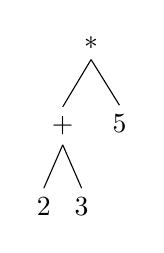
\begin{tikzpicture}
  \Tree [.$*$
    [.$+$
      [.2 ]
      [.3 ]
    ]
    [.5 ]
  ]  
\end{tikzpicture}
\hfill
\begin{minipage}[b]{2.5in}\footnotesize
\begin{verbatim}
  ((2 + 3) * 5)

  2 + 3 * 5

  * + 2 3 5

  2 3 + 5 *
\end{verbatim}
\end{minipage}

\vfill

\hrulefill

\vfill

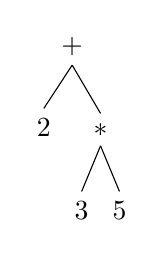
\begin{tikzpicture}
  \Tree [.$+$
    [.2 ]
    [.$*$
      [.3 ]
      [.5 ]
    ]
  ]  
\end{tikzpicture}
\hfill
\begin{minipage}[b]{2.5in}\footnotesize
\begin{verbatim}
  (2 + (3 * 5))

  2 + 3 * 5

  + 2 * 3 5

  2 3 5 * +
\end{verbatim}
\end{minipage}
\end{frame}


\sect{Expressing arithmetic trees}
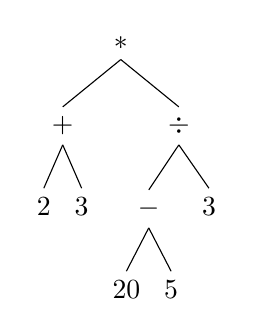
\begin{tikzpicture}
  \Tree [.$*$
    [.$+$
      [.2 ]
      [.3 ]
    ]
    [.$\div$
      [.$-$
        [.20 ]
        [.5 ]
      ]
      [.3 ]
    ]
  ]  
\end{tikzpicture}\hfill
\begin{minipage}[b]{2.5in}\footnotesize
\begin{verbatim}
  ((2 + 3) * ((20 - 5) / 3))

  2 + 3 * 20 - 5 / 3

  * + 2 3 / - 20 5 3

  2 3 + 20 5 - 3 / *
\end{verbatim}
\end{minipage}

\end{frame}


\end{document}
